%===================================== CHAP 8 =================================

\chapter{Results}
Innen hver metode:
\begin{enumerate}
    \item hvordan gjør kapteinen det over alle ukene
    \item hvordan gjør vice-captain det over alle ukene
    \item hvordan gjør substitutions det over alle ukene
    \item plotte total point opp mot justering av penalty variabel
    \item plotte horizon opp mot total points
    \item hvis man legger restriksjon på formasjon. Hvilke formasjon gir mest poeng?
    \item når bruker man de forskjellige chippene, og hvor effektive er de?  
    \item lage et high risk team hvor variansen er høy
    \item Perfect information
\end{enumerate}
-  
- 
-  
-  
-  
- 
- 
-  
-  
\section{Regression Method}
\subsection{Temporary Results}

Table \ref{tab:results_reg_16/17} displays the results from a full run of the model on gameweek 15-25 for the 2016/2017 season. Both the realized points each round, and points when illegal transfers are not accounted for, are presented. Figure \ref{fig:points_15_25_16/17} displays the values plotted for each round.

\begin{figure}[H]
\centering
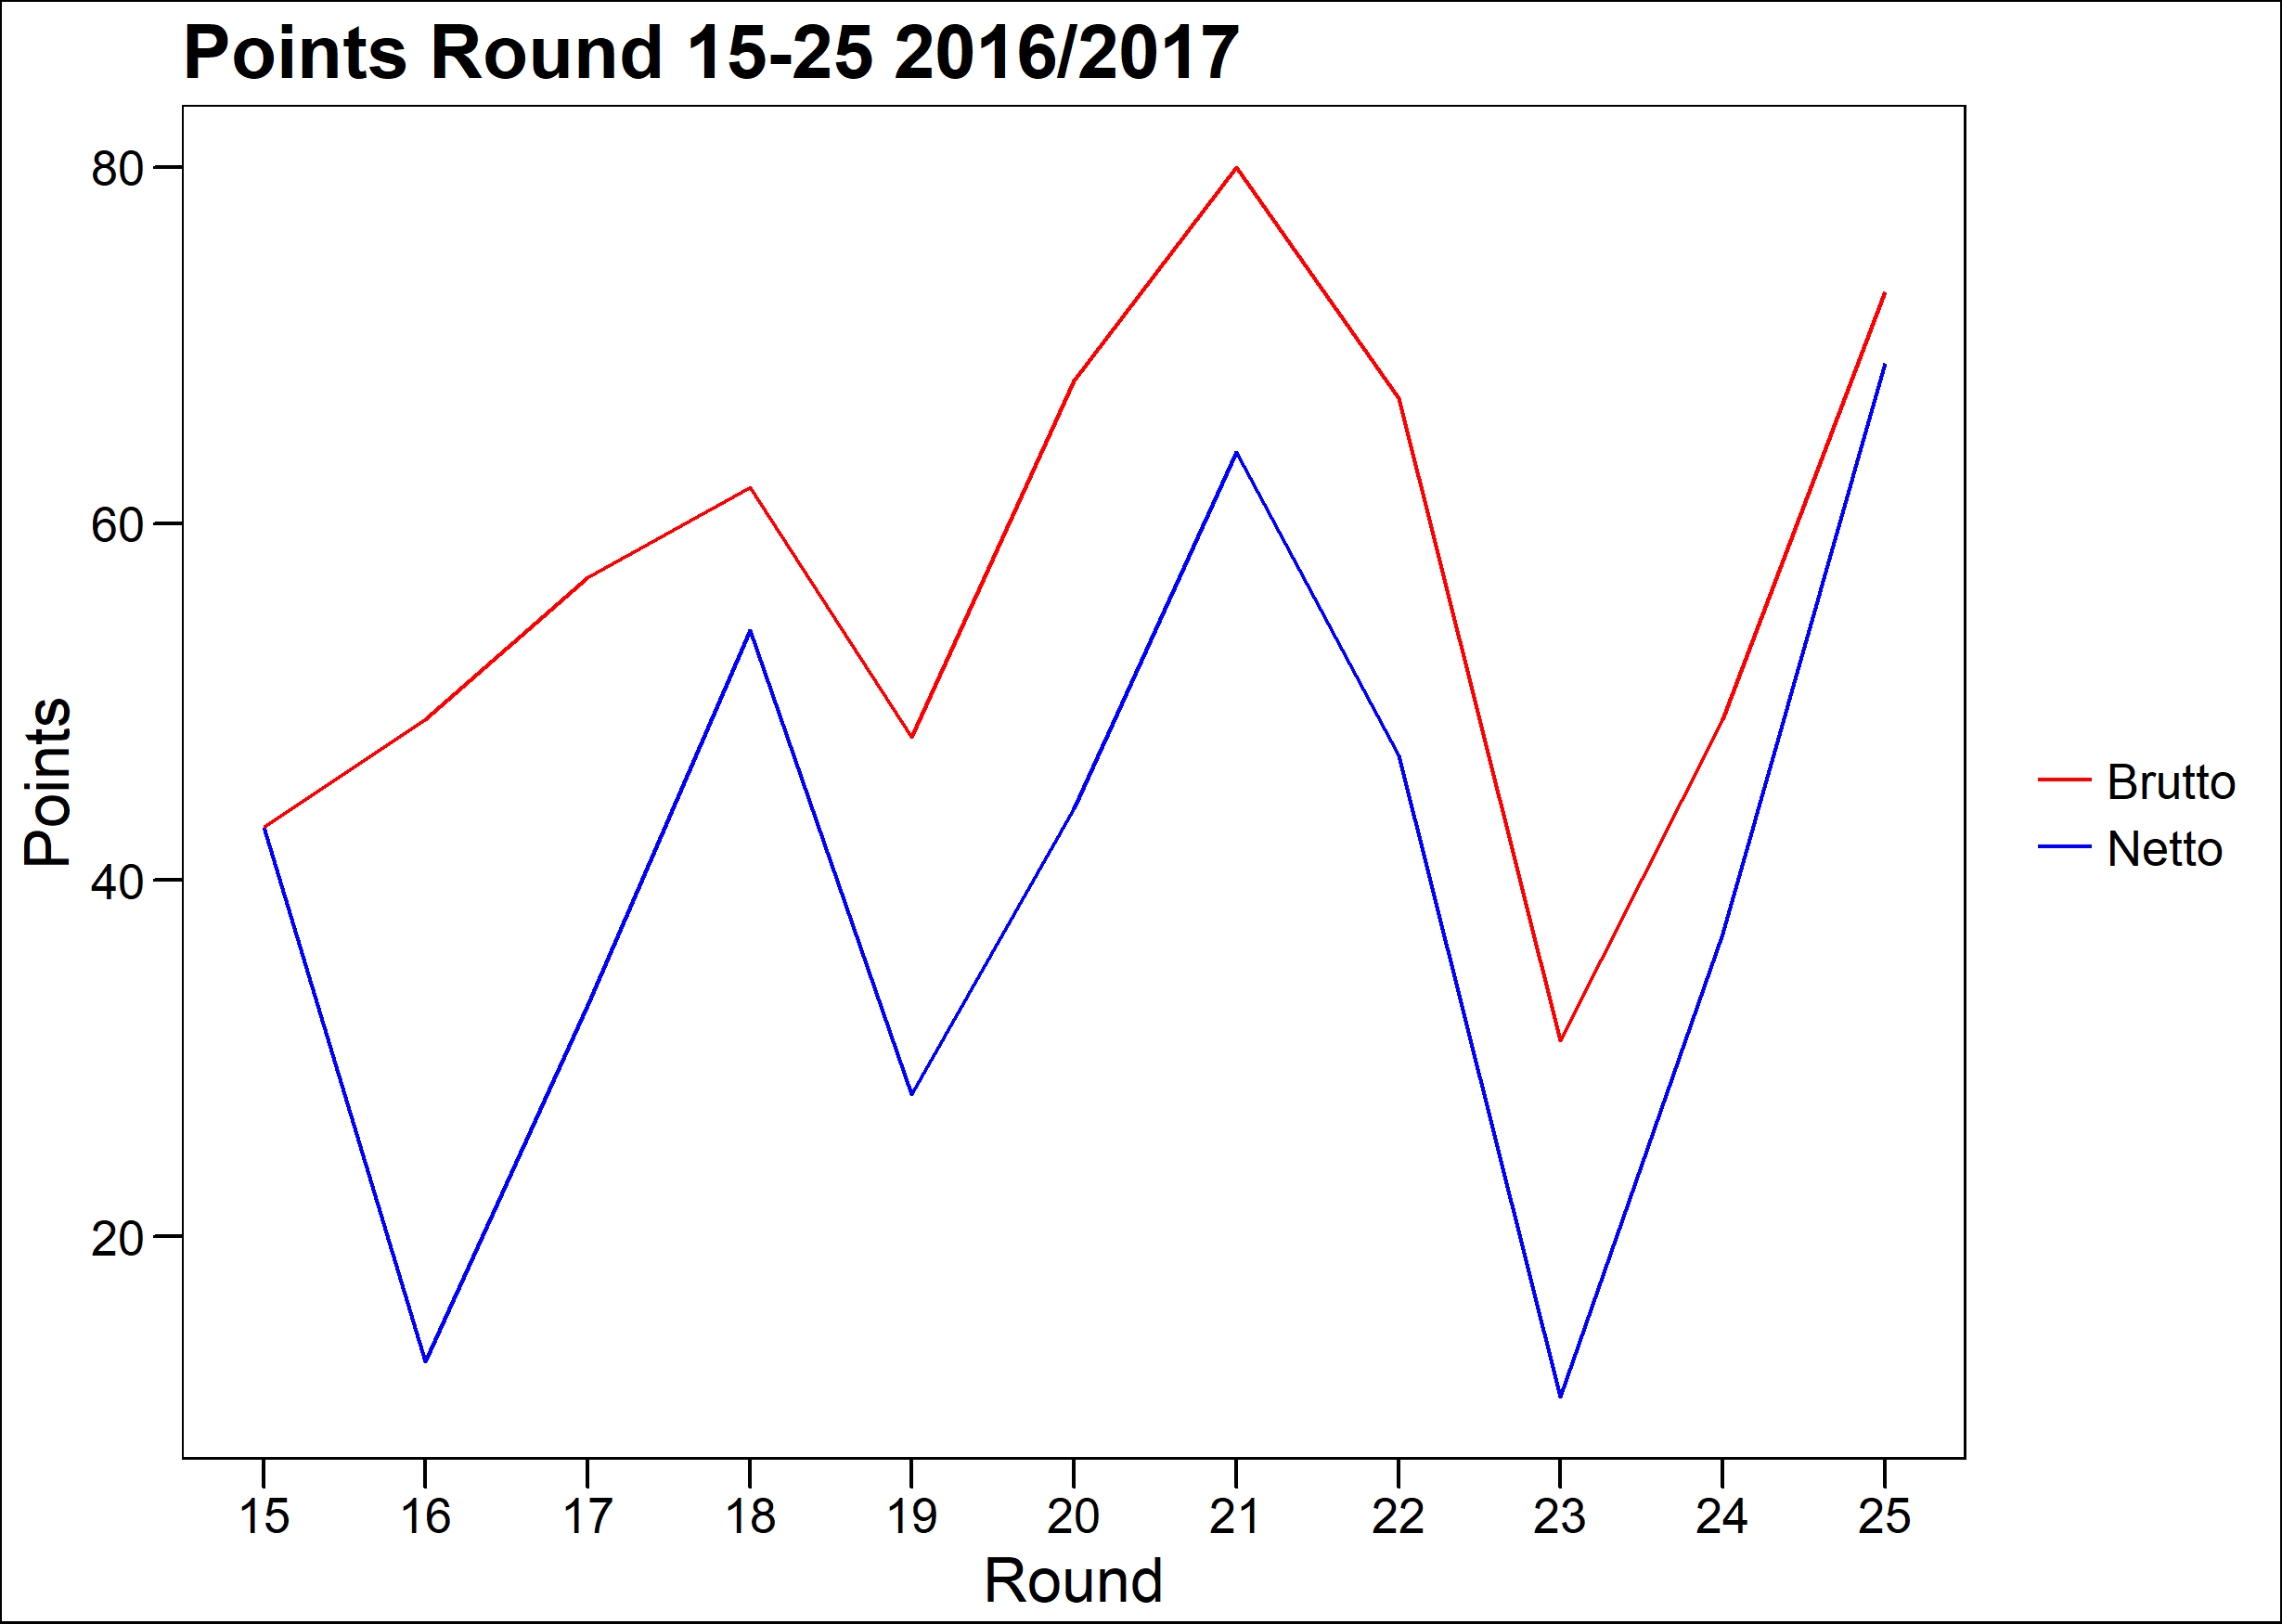
\includegraphics[scale=0.35]{fig/points_15_to_25.png}
 \caption{Plotted realized net and gross points for round 15-25 of the 2016/2017 season.}
\label{fig:points_15_25_16/17}
\end{figure}

\begin{table}[]
\centering
\caption{Realized net and gross points for round 15-25 of the 2016/2017 season.}
\label{tab:results_reg_16/17}
\begin{tabular}{@{}rrr@{}}
\toprule
Round & Points Net & Points Brut \\ 
\midrule
15    & 43     & 43             \\
16    & 13     & 49             \\
17    & 33     & 57             \\
18    & 54     & 62             \\
19    & 28     & 48             \\
20    & 44     & 68             \\
21    & 64     & 80             \\
22    & 47     & 67             \\
23    & 11     & 31             \\
24    & 37     & 49             \\
25    & 69     & 73             \\ 
\end{tabular}
\end{table}


\section{Average Method}
\subsection{Results based on average from previous gameweeks}
\subsection{Advanced average using suggested weightings}
\subsection{Advanced average using ELO-ratings, xG, xA and home advantage}
\section{Odds Method}

